\documentclass[9pt]{article}
\usepackage{natbib}  % or \usepackage{biblatex} for newer bibliography support
\usepackage{enumitem}
\usepackage{latexsym}
\usepackage{amsfonts}
\usepackage{float}
\usepackage{fullpage}
\usepackage{graphicx}
\usepackage{geometry}
\usepackage{pdflscape}
\usepackage{booktabs}
\usepackage{listings}
\usepackage{float}
\usepackage{subfigure}
\usepackage[utf8]{inputenc}

\usepackage{amsmath} % Add the necessary package for the control sequence
\usepackage{setspace} % Add the necessary package for adjusting line spacing
\usepackage{hyperref}
% \usepackage{subcaption}
% Required packages (add to preamble)
\usepackage{listings}
\usepackage{xcolor}
\usepackage{enumitem}
\usepackage{booktabs}
\usepackage{hyperref}
\usepackage{url}
\hypersetup{
    colorlinks=true,
    linkcolor=blue,
    filecolor=magenta,
    urlcolor=cyan
}

% Listings setup for Python code
\lstset{
    language=Python,
    basicstyle=\ttfamily\small,
    keywordstyle=\color{blue},
    commentstyle=\color{green!60!black},
    stringstyle=\color{red},
    showstringspaces=false,
    breaklines=true,
    frame=single,
    numbers=left,
    numberstyle=\tiny,
    numbersep=5pt
}
\geometry{
    left=0.5in,
    right=0.5in,
    top=0.5in,
    bottom=0.5in
}
\newcommand{\N}{\mathcal{N}}
\newcommand{\R}{\mathcal{R}}
\newcommand{\A}{\mathcal{A}}

% Title, author, course, and date
\title{Mid Review Report}
\author{Antara Tewary (G01413546), Homa Haghighi (G01145449), Ankit Kumar (G01436204)}
\date{CS 678, Advanced NLP\\\today}

\begin{document}

% Create the title
\maketitle

\section{Introduction}
\subsection{Task / Research Question Description: }
The task we are addressing involves bridging the language barrier in Python programming for non-English speakers. Python is widely used in education and industry due to its simplicity and English-like syntax, but this presents challenges for learners and developers whose native language is not English. Our project focuses on creating a tool that translates Python's syntax and keywords into multiple human languages, making Python more accessible to non-English speakers. This aims to democratize programming education and foster inclusivity in global computer science learning. 

\subsection{Motivation \& Limitations of Existing Work: }
While Python's design simplifies programming for English speakers, it poses significant obstacles for non-English speakers, as they must not only learn programming concepts but also a foreign language. Several tools, like \textit{CodeInternational}, have attempted to address this issue by translating some parts of programming languages (e.g., comments, string literals). However, these efforts are incomplete and limited in scope, often failing to cover Python's built-in functions and modules or focusing on specific languages. Our project aims to offer a more comprehensive solution, enabling full translation of Python's syntax into various languages. Prior efforts have struggled with language-specific translation issues, such as abbreviations or word order, which our project addresses through advanced translation models and community feedback.

\subsection{Proposed Approach: }
Our approach is to build a universal Python interpreter that translates Python code written in English into multiple human languages. The core contribution is the development of a tool that can translate Python syntax, identifiers and keywords, in real-time, maintaining consistency across different languages. This is done by integrating neural machine translation models and leveraging open-source libraries like Hugging Face. We will also provide a web-based interface using Streamlit, enabling easy access for students and developers to use the tool in both educational and professional settings.  
\subsection{Likely Challenges and Mitigation Strategies: }
    One of the key challenges in this project is ensuring that the translations preserve the technical accuracy and readability of the original Python code. Languages with complex grammatical structures may require more sophisticated translation models. Another challenge is maintaining consistency in translation, especially when handling right-to-left languages or non-Latin scripts. To mitigate these issues, we will rely on native speakers to review and annotate translations, and we will incorporate techniques like domain adaptation and crowd-sourced corrections to improve translation accuracy. If the translation accuracy does not meet expectations, we plan to fine-tune models with additional data and feedback.

\section{Related Work}
    \begin{itemize}
        \item C. Piech and S. Abu-El-Haija, “Human languages in source code: Autotranslation for localized instruction,” in \textit{Proceedings of the Seventh AC Conference on Learning@ Scale}, 2020, pp. 167–174.

        This paper introduces CodeInternational, a tool designed to translate code comments and identifiers across multiple human languages, helping non-English speakers learn programming more easily. The study emphasizes the importance of making code accessible in native languages but primarily focuses on Java and comments/identifiers. Our project differs by aiming to translate the entire Python syntax, not just comments or identifiers, providing a more comprehensive solution for Python programming education in non-English languages.
        
        \item A. Hindle, E. T. Barr, Z. Su, M. Gabel, and P. Devanbu, “On the naturalness of software,” in \textit{Proceedings of the 34th International Conference on Software Engineering}, ser. ICSE ’12. IEEE Press, 2012, p. 837–847.
        
        This paper explores how code, like natural language, follows repetitive patterns, which can be modeled using statistical language models such as n-grams. The work applies these models to tasks like code completion and suggests that programming languages are predictable. While this research focuses on enhancing software development efficiency, our project applies similar language models but aims to address the language accessibility challenge by translating Python syntax for non-English speakers.
        
        \item M. White, C. Vendome, M. Linares-Vásquez, and D. Poshyvanyk, “Toward deep learning software repositories,” in \textit{Proceedings of the 12th Working Conference on Mining Software Repositories}, ser. MSR ’15. IEEE Press, 2015, p. 334–345.
        
        The authors demonstrate the application of deep learning models to analyze software repositories and improve tasks like bug prediction and code completion. Their deep learning models perform well on large software corpora. Our project builds on these deep learning concepts but uses them to handle the translation of Python's structure and syntax into multiple human languages, a task that extends beyond improving code completion.
        
        \item D. Guo, S. Lu, N. Duan, Y. Wang, M. Zhou, and J. Yin, “UniXcoder: Unified cross-modal pre-training for code representation,” in \textit{Proceedings of the 60th Annual Meeting of the Association for Computational Linguistics (Volume 1: Long Papers)}. Dublin, Ireland: Association for Computational Linguistics, May 2022, pp. 7212–7225.
        
        UniXcoder proposes a model that utilizes code comments and abstract syntax trees (AST) to improve code representation and generation across different programming tasks. This work focuses on enhancing programming tasks like code completion through multi-modal data. In contrast, our project focuses on the translation of Python's syntax into human languages, leveraging multi-modal data like AST for language translation and accessibility rather than improving programming performance.
    \end{itemize}

\section{Methodology}

Our project, PyLinguist, aims to create a tool that translates Python code from English to other human languages, focusing initially on Hindi. Our methodology consists of the following structured approach:
\subsection{Dataset Acquisition and Preparation}
For our research, we leverage a comprehensive Python code dataset from Hugging Face, encompassing 559,515 code examples. This dataset provides a rich collection of complete Python code snippets, associated documentation, and diverse programming constructs including functions, loops, and conditional statements. The dataset follows a structured format containing three main components: code snippets in the output field, corresponding task descriptions, and system prompts.

\begin{lstlisting}
{
    'output': [Python code snippets],
    'instruction': [task descriptions],
    'system': [system prompts]
}
\end{lstlisting}

\subsection{Code Component Parsing and Tokenization}
Our approach begins with breaking down Python code into its fundamental components for targeted translation. The parsing process addresses two primary categories: syntax elements and natural language elements. The syntax elements comprise Python keywords (such as if, for, while), built-in functions (print, len, range), and various operators and delimiters. The natural language elements include comments, string literals, and variable identifiers.

To illustrate our parsing process, consider the following example:

\begin{lstlisting}
# Example of component breakdown
original_code = """
for i in range(5):  # Loop 5 times
    print(i)        # Print current number
"""
# Breaks down into:
components = {
    'keywords': ['for', 'in'],
    'built_ins': ['range', 'print'],
    'variables': ['i'],
    'comments': ['Loop 5 times', 
                'Print current number']
}
\end{lstlisting}

\subsection{Translation System Development}
Our translation system employs a two-phase approach. The first phase establishes a baseline using the Google Translate API to create a parallel English-Hindi corpus for Python components. This process involves systematic translation of Python keywords, built-in functions, and common programming constructs, ensuring consistent mapping between English and Hindi equivalents.
\begin{figure}[h]
    \centering
    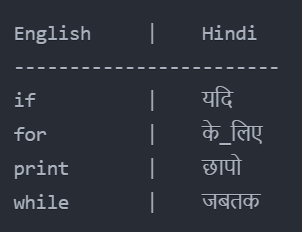
\includegraphics[width=0.2\textwidth]{english-hindi-translation-mapping.png}
    \caption{Translation Mapping Overview}
    \label{fig:translation_system}
\end{figure}
In the second phase, we develop a custom model based on pre-trained language models such as BERT or LLAMA. This model is specifically fine-tuned using our parallel corpus of English-Hindi code translations. The training process focuses on preserving both the syntactic structure of the code and its semantic meaning, with particular attention to programming-specific language patterns.

\subsection{Implementation Flow}
The implementation follows a systematic pipeline that begins with raw English Python code as input. The code undergoes tokenization and parsing to identify its constituent components. We then apply our translation system, using direct mapping for technical elements like keywords and built-in functions, while employing neural translation for natural language components such as comments and documentation. The final step involves reconstructing the code while maintaining Python's syntactic rules, resulting in functionally equivalent Hindi code.

\subsection{Evaluation Strategy}

Our evaluation methodology encompasses three main components: technical validation, human evaluation, and continuous documentation.

\subsubsection{Technical Validation}
We will implement rigorous syntax validation to ensure the translated code maintains Python's structural integrity. Each translated code segment will be automatically tested for proper execution, maintaining identical functionality to its English counterpart.

\subsubsection{Human Evaluation}
Native Hindi-speaking programmers will serve as our primary evaluators, providing insights through structured assessment tasks. We will measure code comprehension speed and accuracy through practical programming exercises. Participants will complete code modification tasks and rate their experience on a five-point scale, offering quantitative metrics for the translation effectiveness.

To gather comprehensive feedback, participants will engage in code reading exercises and practical programming tasks using the translated code. Their experiences and challenges will be documented through structured surveys, providing valuable insights for system improvement.

\subsubsection{Documentation and Iteration}
Our iterative improvement process relies on systematic documentation of translation patterns and edge cases. We maintain detailed logs of all translations and their associated challenges, enabling consistent version control of improvements. Regular model updates are implemented based on both technical performance metrics and human feedback, ensuring continuous enhancement of the translation system.
\section{Experiments}

\subsection{Dataset}
Our experiments utilize the Python code dataset available on Hugging Face:
\url{https://huggingface.co/datasets/jtatman/python-code-dataset-500k?row=0}


\subsection{Implementation}
The complete implementation of PyLinguist is available on GitHub:
\url{https://github.com/StringAna/PyLinguist.git}

\noindent To advance PyLinguist, our experimental approach consists of the following phases:
\subsection{Dataset Creation}
Our dataset development focuses on essential Python code elements including comments, variable declarations, conditional statements, and loop structures. Using Google Translate API, we create a parallel corpus by translating each English component to Hindi, establishing a foundation for model training and evaluation.

\subsection{Model Selection and Training}
We begin with pre-trained language models, specifically BERT or LLaMA, as our base models. The fine-tuning process uses our custom parallel dataset, with particular emphasis on Hindi syntax accuracy and semantic preservation. Our training prioritizes the effective translation of essential Python constructs while maintaining code functionality.

\subsection{Evaluation Setup}
Our evaluation combines both quantitative and qualitative metrics. For quantitative assessment, we employ BLEU scores to measure translation fidelity and conduct systematic comparisons with reference translations. The qualitative evaluation involves native Hindi-speaking programmers who assess translation quality, practical usability, and syntactic correctness of the translated code.

\subsection{Error Analysis}
The error analysis phase systematically identifies both successful translations and challenging cases. We examine translation quality across varying complexity levels of Python constructs and use these insights to guide iterative improvements. This systematic approach helps refine our model's performance and ensures reliable code translation across different programming contexts.

\section{Conclusion}
Our project, PyLinguist, contributes a novel approach to translating Python code syntax, keywords, and comments into Hindi, with plans to expand into other languages to enhance programming accessibility globally. Starting with a custom Hindi dataset, we fine-tune pre-trained language models to address the unique challenges of programming language translation. This work establishes a foundation for future multilingual support, promoting inclusivity in coding education and development. 

\bibliographystyle{ieeetr}  % or other styles like 'ieeetr', 'acm', etc.

\begin{thebibliography}
    \bibitem"Towards a Universal Python: Translating the Natural Modality of Python into Other Human Languages" by \textit{Otten, Joshua and Anastasopoulos, Antonios and Moran, Kevin P}, [Online]. Available: \url{https://nlp.cs.gmu.edu/publication/otten-etal-23-unipy/} [Accessed October 23, 2024]
\end{thebibliography}


\end{document}